\documentclass{article}
\usepackage[T1]{fontenc}
\usepackage{lmodern}
\usepackage[polish]{babel}
\usepackage{graphicx}
\usepackage{float}
\usepackage{hyperref}
\usepackage{amsmath}
\usepackage{listings}
\usepackage{xcolor}

\usepackage[a4paper, margin=2.54cm]{geometry}

\lstset{
  basicstyle=\ttfamily,
  columns=fullflexible,
  frame=single,
  breaklines=true,
  postbreak=\mbox{\textcolor{red}{$\hookrightarrow$}\space},
  literate=%
    {ą}{{\k a}}1
    {Ą}{{\k A}}1
    {ę}{{\k e}}1
    {Ę}{{\k E}}1
    {ó}{{\' o}}1
    {Ó}{{\' O}}1
    {ś}{{\' s}}1
    {Ś}{{\' S}}1
    {ł}{{\l}}1
    {Ł}{{\L}}1
    {ż}{{\. z}}1
    {Ż}{{\. Z}}1
    {ź}{{\' z}}1
    {Ź}{{\' Z}}1
    {ć}{{\' c}}1
    {Ć}{{\' C}}1
    {ń}{{\' n}}1
    {Ń}{{\' N}}1
}

\title{Praca domowa 7\\Porównanie algorytmu roju i genetycznego}
\author{Damian Jankowski s188597}

\begin{document}

\maketitle

\section{Wstęp}

Celem pracy domowej było porównanie algorytmu roju 
cząstek (PSO) oraz algorytmu genetycznego (GA) w wybranym problemie.

Zdecydowałem się na problem plecakowy, który polega na wybraniu
zbioru przedmiotów o określonej wartości i wadze, tak aby
maksymalizować wartość przedmiotów, a jednocześnie nie przekroczyć
określonej wagi plecaka.

\section{Opis algorytmów}


\subsection{Algorytm roju cząstek}

Algorytm roju cząstek (Particle Swarm Optimization, PSO) 
jest metaheurystyką inspirowaną zachowaniem stad i rojów w naturze. 
Algorytm składa się z populacji cząstek, gdzie każda cząstka reprezentuje 
jedno potencjalne rozwiązanie problemu. Każda cząstka porusza się w 
przestrzeni rozwiązań, posiadając swoją pozycję oraz prędkość.

Algorytm PSO opiera się na iteracyjnym przemieszczaniu cząstek w 
poszukiwaniu optymalnego rozwiązania. Cząstki zmieniają swoje pozycje 
i prędkości w oparciu o najlepsze znalezione dotychczas rozwiązanie dla
danej cząstki (lokalne najlepsze rozwiązanie) oraz najlepsze znalezione 
rozwiązanie wśród wszystkich cząstek (globalne najlepsze rozwiązanie).

Podczas iteracji, cząstki poruszają się w przestrzeni rozwiązań, 
aktualizując swoje pozycje i prędkości na podstawie zdefiniowanych równań.

W kontekście problemu plecakowego, algorytm PSO poszukuje kombinacji przedmiotów 
optymalnie umieszczonych w plecaku, tak aby maksymalizować wartość przedmiotów, 
jednocześnie nie przekraczając określonej wagi plecaka. Cząstki w tym przypadku 
reprezentują różne kombinacje produktów, a optymalne rozwiązanie polega na znalezieniu 
cząstki, której kombinacja przedmiotów ma najwyższą wartość.


\subsection{Algorytm genetyczny}

Algorytm genetyczny (Genetic Algorithm, GA) jest metaheurystyką inspirowaną 
procesem ewolucji biologicznej. Algorytm operuje na populacji rozwiązań, które 
są reprezentowane przez struktury zwane chromosomami. Chromosomy składają się 
z genów, które zawierają informacje o cechach rozwiązania.

Algorytm genetyczny operuje na populacji, gdzie każde rozwiązanie jest kodowane 
jako chromosom. Algorytm składa się z kilku kroków, takich jak selekcja, krzyżowanie, mutacja i ewaluacja.

Selekcja polega na wyborze najlepszych rozwiązań z populacji na podstawie funkcji celu. 
Następnie, wybrane rozwiązania są krzyżowane, co polega na wymianie części informacji 
genetycznej pomiędzy dwoma chromosomami, aby stworzyć potomstwo. Krzyżowanie ma na 
celu zwiększenie różnorodności populacji i wprowadzenie nowych kombinacji genetycznych.

Mutacja polega na losowej zmianie pewnych genów w chromosomie, co pomaga w eksploracji 
nowych obszarów przestrzeni poszukiwań. Po krzyżowaniu i mutacji, oceniana jest jakość 
nowo powstałego potomstwa za pomocą funkcji celu. Jeśli potomstwo ma lepszą jakość niż 
pewne osobniki w populacji, zastępuje je.

Algorytm podobnie jak algorytm roju cząstek kontynuuje iteracje, aż do osiągnięcia 
zadowalającego rozwiązania lub spełnienia warunku stopu.

\section{Porównanie}

By porównać działanie algorytmów zaimplementowałem 
najpierw generator instancji problemu plecakowego, który
tworzy 20 przedmiotów o losowej wadzie i wartości. Następnie
zaimplementowałem algorytm roju cząstek oraz algorytm genetyczny,
które rozwiązują ten problem w czasie 100 iteracji.

Dla sprawdzenia działania algorytmów, zaimplementowałem
również algorytm brute-force, który sprawdza wszystkie możliwe
kombinacje przedmiotów i wybiera tą, która ma największą wartość
i mieści się w plecaku.

\subsection{Wyniki}

Dla następującego plecaka:

\begin{lstlisting}
    Plecak o pojemnosci:  2000
    Produkty:
    Nazwa           Wartosc Waga
    Produkt 1        296     347
    Produkt 2        962     210
    Produkt 3        663     153
    Produkt 4        676     179
    Produkt 5        484     466
    Produkt 6        706     146
    Produkt 7        261     453
    Produkt 8        163     486
    Produkt 9        752     228
    Produkt 10       878     394
    Produkt 11       987     427
    Produkt 12       828     394
    Produkt 13       333     370
    Produkt 14       797     446
    Produkt 15       515     382
    Produkt 16       669     146
    Produkt 17       328     329
    Produkt 18       335     112
    Produkt 19       379     436
    Produkt 20       210     327
\end{lstlisting}

\subsection{Brute force}

Algorytm brute-force znalazł następujące rozwiązanie:

\begin{lstlisting}
    Brute force:
    Najlepsza wartosc:  6628
    Najlepsza pozycja:  [0, 1, 1, 1, 0, 1, 0, 0, 1, 1, 1, 0, 0, 0, 0, 1, 0, 1, 0, 0]
\end{lstlisting}

\subsection{Algorytm roju cząstek}
Algorytm roju cząstek znalazł następujące rozwiązanie:

\begin{lstlisting}
    Algorytm roju czastek:
    Najlepsza wartosc:  6628
    Najlepsza pozycja:  [0, 1, 1, 1, 0, 1, 0, 0, 1, 1, 1, 0, 0, 0, 0, 1, 0, 1, 0, 0]
\end{lstlisting}

\begin{figure}[H]
    \centering
    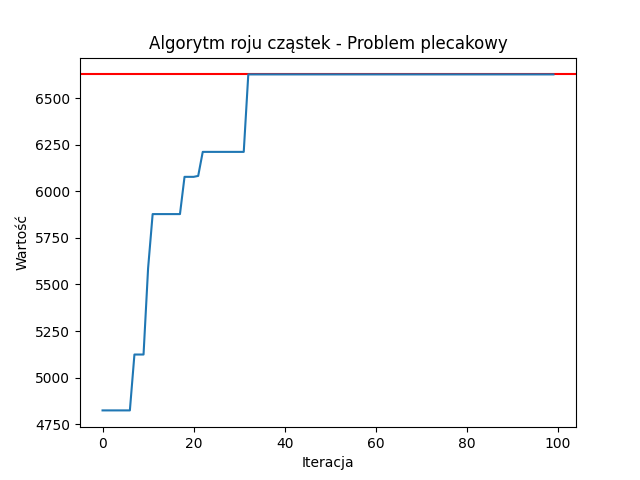
\includegraphics[width=0.8\textwidth]{pso.png}
    \caption{Wykres wartości plecaka w zależności od iteracji dla algorytmu roju cząstek}
\end{figure}

\subsection{Algorytm genetyczny}
Natomiast algorytm genetyczny znalazł następujące rozwiązanie:

\begin{lstlisting}
    Algorytm genetyczny:
    Najlepsza wartosc:  6628
    Najlepsza pozycja:  [0, 1, 1, 1, 0, 1, 0, 0, 1, 1, 1, 0, 0, 0, 0, 1, 0, 1, 0, 0]
\end{lstlisting}

\begin{figure}[H]
    \centering
    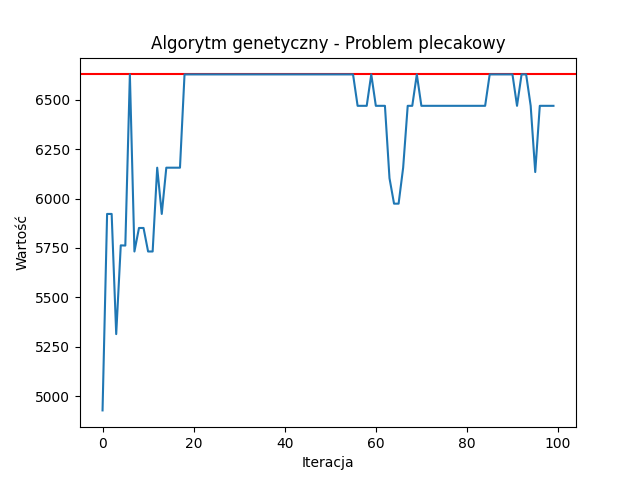
\includegraphics[width=0.8\textwidth]{ga.png}
    \caption{Wykres wartości plecaka w zależności od iteracji dla algorytmu genetycznego}
\end{figure}

\section{Wnioski}

W przypadku algorytmu roju cząstek, wartość plecaka dąży do wartości optymalnej
mniej chaotycznie niż w przypadku algorytmu genetycznego. Po osiągnięciu niej
wartości plecaka nie zmieniają się już i pozostają na stałym poziomie.

Algorytm genetyczny osiąga wartość optymalną szybciej niż algorytm roju cząstek,
jednakże nie jest w stanie jej utrzymać i wartość plecaka zaczyna oscylować.

Wybór algorytmu zależy od tego, czy zależy nam na szybkim, choć nie pewnym
znalezieniu rozwiązania czy na stabilnym dążeniu do niego. W przypadku algorytmu roju (PSO)
dzięki ciągłej aktualizacji pozycji cząstek, algorytm jest w stanie
znaleźć globalne optimum. Wadą takiego rozwiązania jest
możliwość wymogu większej liczby iteracji, aby znaleźć rozwiązanie.

Algorytm genetyczny (GA) jest w stanie znaleźć rozwiązanie szybciej niż PSO oraz
dzięki mechanizmom selekcji, krzyżowania i mutacji, eksplorować 
różne kombinacje populacji. Natomiast może być podatny na utknięcie w lokalnym
optimum oraz być skłonny do oscylacji wokół wartości optymalnej.



\section{Kod programu}

\lstinputlisting[
language=python,  
basicstyle=\small\tt,
keywordstyle=\color{blue},
backgroundcolor=\color{cyan!10}
]{main.py}

\end{document}

